% !TEX root=report.tex
\section{Features} \label{sec:features}

The featurization function $\Phi(s,h,r)$ maps properties of a couch request $r$ from surfer $s$ to host $h$ to a real-dimensional $D$-vector.
The properties we care about include structured personal information such as age, gender, languages spoken, countries lived in, countries traveled to, and so on.
Additionally, we would like to use user interests, extracted from free form text on their profiles, and their status and activity on the website, e.g. the number of references, number of friends, or message response rate.

We developed a general approach for dealing with a wide variety of features.
For each feature, we construct a histogram whose boundaries are determined by the inverse distribution of values in the training set.
Using this mapping from value to bin we vectorize each feature by mapping it to a binary vector with the constraint of summing to $1$ (e.g. $age=27$ to $b=[0,0,0,1,0,\dots]^T$).
Since our feature $\Phi(s,h)$ is based on both the surfer $s$ and the host $h$, the final feature includes this binary vector for each of them, as well as the outer product between the two, $b_s b_h^T$.

The reason for the outer product feature is to capture potential preference combinations.
For example, we are able to model that hosts between $21$ and $25$ years old prefer surfers of the same age, while hosts over $60$ don't have a particular preferences in this regard (as an example).
Other example inlude capturing affinities between genders, countries, spoken languages, certain interest groups, etc.

In addition to these cross-product preference features, we include additional unary features, such as the number of languages in common, and features relating to reputation.
The final feature vector is quite sparse.

\subsection{User interests} \label{subsec:user_interests}

We also extract ``interests'' features from free-form user profile text as additional signal to the feature vector.
Guided by \cite{Liu2005,Liu2006,Cantador2011}, we form a graph of profile terms found in user profiles.
The edge strength between two terms is proportional to the number of times the terms co-occur in user profiles.
This measure is of course biased toward frequently-occuring terms.
We use a normalization scheme that accounts for this, and the edge strength between $w_1$ and $w_2$ is determined as
\begin{eqnarray}
\frac{P(w_1,w_2)}{2} (\frac{1}{P(w_1)} + \frac{1}{P(w_2)})
\end{eqnarray}

On this graph, we are able to find clusters of common terms, which we refer to as ``interests.''
We use an algorithm from \cite{Blondel2008}, implemented in open-source software\footnote{Gephi at \url{http://gephi.org}, based on GraphViz.}
An example of such a clustered graph is given in ~\autoref{fig:interest_graph}.

\begin{figure}[ht]
\centering
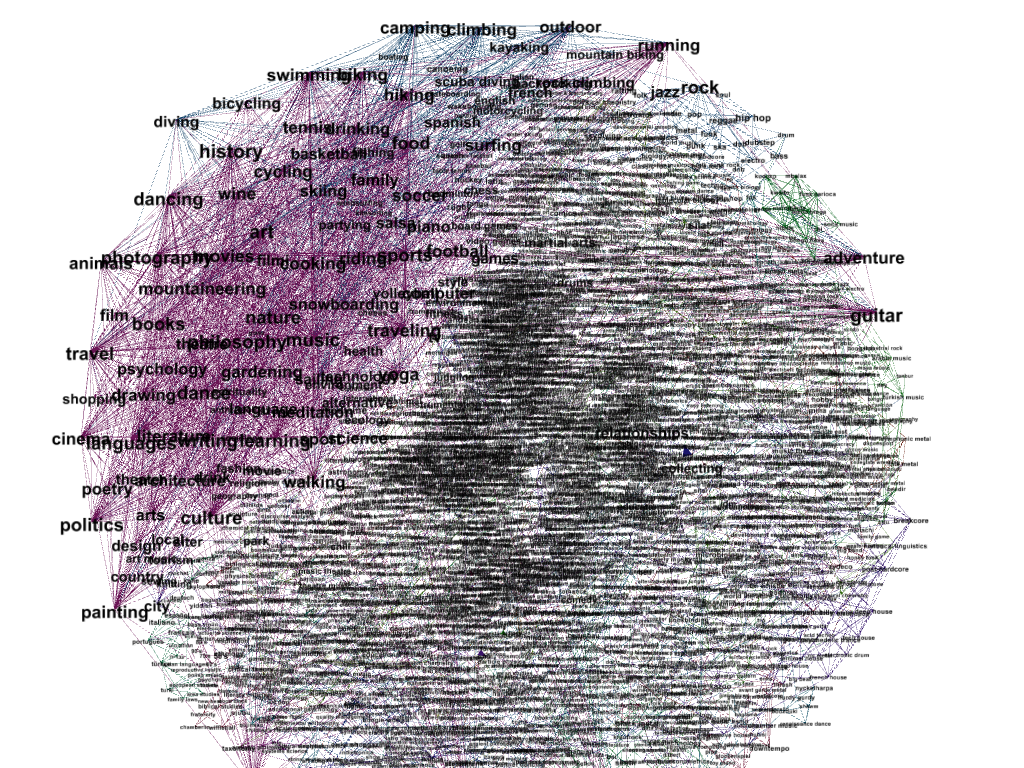
\includegraphics[width=1\linewidth]{figures/interest_graph.png}
\caption{Graph of terms occuring in free-form user profile text, with ``interest'' clustered in color.}
\label{fig:interest_graph}
\end{figure}

We vectorize a user's interests to a binary vector $i$ that has no constraint of summing to $1$, e.g. a user expressing clusters $2$ and $4$ out of $C=5$ total clusters would have $i=[0,0,1,0,1]$.
We pick the number of clusters $C$ by hand, and include the cross-product feature (defined as before) into the final feature $\Phi(s,h)$.

